%% =====================================================================
%%  Simulacija odljeva mozgova u europskim zemljama
%% =====================================================================
\documentclass[11pt,a4paper]{article}

\usepackage[utf8]{inputenc}
\usepackage[T1]{fontenc}
\usepackage[croatian]{babel}
\usepackage{lmodern}
\usepackage{geometry}
\usepackage{booktabs}
\usepackage{amsmath}
\usepackage{xcolor}
\usepackage{hyperref}
\usepackage{fancyhdr}
\usepackage[nobottomtitles*]{titlesec}
\usepackage{enumitem}
\usepackage{mdframed}
\usepackage{caption}
\usepackage{graphicx}
\usepackage{float}

\geometry{top=2.2cm, bottom=2.2cm, left=2.6cm, right=2.2cm, headheight=14pt}

\definecolor{primaryblue}{RGB}{0,62,116}
\definecolor{accentblue}{RGB}{0,120,212}
\definecolor{lightgray}{RGB}{245,245,245}
\definecolor{darkgray}{RGB}{80,80,80}
\definecolor{warnred}{RGB}{180,30,30}
\definecolor{okgreen}{RGB}{20,130,60}
\definecolor{boxborder}{RGB}{180,200,220}

\titleformat{\section}{\large\bfseries\color{primaryblue}}{\thesection}{0.8em}{}%
  [\vspace{-4pt}\rule{\linewidth}{0.4pt}]
\titleformat{\subsection}{\normalsize\bfseries\color{accentblue}}{\thesubsection}{0.7em}{}
\titlespacing{\section}{0pt}{12pt}{5pt}
\titlespacing{\subsection}{0pt}{7pt}{2pt}

\pagestyle{fancy}
\fancyhf{}
\fancyhead[L]{\small\textcolor{darkgray}{Simulacija odljeva mozgova u europskim zemljama}}
\fancyhead[R]{\small\textcolor{darkgray}{Petar Prenc, 2026.}}
\fancyfoot[C]{\small\thepage}
\renewcommand{\headrulewidth}{0.4pt}

\setlength{\parskip}{5pt}
\setlength{\parindent}{0pt}

\hypersetup{colorlinks, linkcolor=accentblue, urlcolor=accentblue,
  pdftitle={Simulacija odljeva mozgova}, pdfauthor={Petar Prenc}}
\captionsetup{font=small, labelfont=bf}

%% =====================================================================
\begin{document}

%% ============================  NASLOVNICA  ===========================
\begin{titlepage}
\newgeometry{top=0cm,bottom=0cm,left=0cm,right=0cm}
\noindent
% Gornji obojeni blok
\colorbox{primaryblue}{\parbox{\paperwidth}{%
  \vspace{2.6cm}
  \hspace{2.6cm}%
  \begin{minipage}{0.82\paperwidth}
    {\color{white}\footnotesize\bfseries\MakeUppercase{Sveučilišni diplomski studij}}\\[0.4em]
    {\color{white!70!primaryblue}\footnotesize Kolegij modeliranja i simulacije  - projektna dokumentacija}\\[2.2em]
    {\color{white}\fontsize{32}{38}\bfseries\selectfont Odljev mozgova\\[0.15em]
     u europskim zemljama}\\[1em]
    {\color{white!80!primaryblue}\large Analiza emigracije visokoobrazovanog kadra\\
     i učinci mjera javne politike}
  \end{minipage}%
  \vspace{2.2cm}
}}%
% Bijeli razdjelnik s akcentom
\noindent\colorbox{accentblue}{\parbox{\paperwidth}{\vspace{3pt}}}%
\vspace{2.2cm}

% Srednji dio  - meta podaci
\hspace{2.6cm}%
\begin{minipage}{0.4\linewidth}
  {\small\color{darkgray}\MakeUppercase{\bfseries Autor}}\\[4pt]
  {\large\bfseries Petar Prenc}\\[1.6em]
  {\small\color{darkgray}\MakeUppercase{\bfseries Datum}}\\[4pt]
  {\large lipanj 2026.}
\end{minipage}%
\hfill
\begin{minipage}{0.38\linewidth}
  {\small\color{darkgray}\MakeUppercase{\bfseries Metoda simulacije}}\\[4pt]
  {\large Sustavna dinamika}\\
  {\small\color{darkgray}\textit{System Dynamics}}\\[1.6em]
  {\small\color{darkgray}\MakeUppercase{\bfseries Implementacija}}\\[4pt]
  {\large R\,/\,Shiny}\\
  {\small\color{darkgray}\textit{15 europskih zemalja · horizont do 2055.}}
\end{minipage}%
\hspace{1cm}

\vfill
\hspace{2.6cm}%

\vspace{1.2cm}
\restoregeometry
\end{titlepage}

%% =====================================================================
\section{Opis sustava i područje primjene}

\textbf{Odljev mozgova} (\textit{brain drain}) označava trajnu emigraciju visokoobrazovanih radnika  - liječnika, inženjera, informatičara, ekonomista  - iz manje razvijenih zemalja prema razvijenijim destinacijama. Za Hrvatsku i slične tranzicijske ekonomije ovaj fenomen nije tek demografski podatak: svaki stručnjak koji ode sa sobom nosi i porezne prihode, inovacijski kapacitet i vrijednost javnih investicija uloženih u njegovo školovanje.

Od ulaska Hrvatske u EU 2013.\ sloboda kretanja radne snage postala je dvosječni mač  - isti zakon koji omogućuje uvoz strane stručnosti domaće stručnjake šalje prema Njemačkoj, Irskoj i skandinavskim zemljama, privučene plaćama i tri do pet puta višim od domaćih. Problematičnost situacije pojačava \textbf{samopojačavajuća logika}: što više stručnjaka ode, to su domaće plaće niže, javne usluge lošije i zemlja manje privlačna za preostale  - što potiče daljnji odlazak.

\textbf{Cilj projekta} jest kvantificirati tu logiku kroz računalnu simulaciju: koliko dugoročno košta neaktivnost, koliko vrijedi rana intervencija i koje mjere imaju najveći povrat ulaganja. Simulacija pokriva \textbf{15 europskih zemalja}  - od bugarskog i rumunjskog dna do irskog i njemačkog vrha ljestvice  - kako bi se tranzicijskim ekonomijama pokazalo što im predstoji i kamo mogu stići.

Model prati četiri međuovisna elementa sustava: \textbf{visokoobrazovanu radnu snagu} (koliko ih je, koliko stigne, koliko ode), \textbf{gospodarski rast} (BDP per capita kao mjera životnog standarda), \textbf{kvalitetu zdravstvenog sustava} (posebno osjetljivog na odljev liječnika i medicinskih sestara) i \textbf{razvoj IT sektora} (koji gubi investicijski zamah kad odlaze programeri i inženjeri).

Model je namijenjen kreatorima politika za procjenu mjera zadržavanja kadrova, ministarstvima za dugoročno planiranje obrazovnih kapaciteta i regionalnim agencijama za optimizaciju korištenja EU fondova.

%% =====================================================================
\section{Vrsta simulacije i simulacijski jezik}

\subsection*{Zašto sustavna dinamika?}

Problem odljeva mozgova ne može se analizirati statičkim alatima. Radi se o sustavu koji se mijenja kroz \textbf{desetljeća}, u kojemu odluke i posljedice nisu trenutne, a varijable su međusobno isprepletene povratnim vezama. Primjerice: niže plaće potiču emigraciju, emigracija smanjuje poreznu bazu, manja porezna baza smanjuje javne investicije, manji javni rashodi usporavaju rast plaća  - krug se zatvara.

Za ovakve probleme razvijena je metodologija \textbf{sustavne dinamike} (\textit{System Dynamics}), pristup koji su 1950-ih na MIT-u razvili Jay Forrester i njegovi suradnici. Osnovna ideja je jednostavna: sustav se opisuje kao skup \textbf{zaliha} (npr.\ broj visokoobrazovanih radnika, razina BDP-a) i \textbf{tokova} koji te zalihe pune ili prazne (diplomirci koji ulaze u tržište rada, emigranti koji ga napuštaju). Povratne veze između varijabli ključne su za razumijevanje zašto sustavi ponekad ne reagiraju onako kako bi kreatori politika očekivali.

\subsection*{Tehnički okvir}

Simulacija je implementirana u \textbf{programskom jeziku R} i dostupna je kao interaktivna web-aplikacija izrađena u \textbf{Shiny} okviru, što znači da je dostupna u pregledniku bez potrebe za instalacijom softvera. Model računa s \textbf{kvartalnim korakom} (svaki korak = tri mjeseca) kroz vremenski horizont od \textbf{2025.\ do 2055.\ godine}.

Radi procjene pouzdanosti rezultata provedena je i \textbf{analiza osjetljivosti}: model je pokrenut 80 puta s nasumično variranim pretpostavkama ($\pm 30\,\%$ od baznih vrijednosti). Ako se zaključci ponavljaju u gotovo svim scenarijima, model je robustan  - a rezultati pokazuju upravo to.

Aplikacija korisnicima omogućuje interaktivno postavljanje pitanja: \textit{Što se dogodi ako Hrvatska sutra uvede porezne olakšice? Što ako to učini tek za pet godina? Što ako EU fondovi ostanu na razini 2\,\% BDP-a?}

%% =====================================================================
\section{Prikupljeni podaci}

\subsection*{Što smo mjerili i odakle}

Sve polazne vrijednosti temelje se na \textbf{službenim statističkim podacima} iz 2023./2024.\ godine, prilagođenim kao procjena za baznu godinu simulacije (\textbf{2025.}):

\begin{itemize}[noitemsep, topsep=3pt]
  \item \textbf{Eurostat}  - BDP per capita, stope emigracije, rashodi za obrazovanje, struktura zaposlenih po sektorima.
  \item \textbf{World Bank World Development Indicators}  - relativne razine plaća u odnosu na EU prosjek, udio visokoobrazovanih u radnoj snazi.
  \item \textbf{Državni zavod za statistiku RH (DZS)}  - detaljniji podaci za Hrvatsku kao primarno promatranu zemlju.
\end{itemize}

Za svaku od 15 zemalja prikupljeno je šest ključnih pokazatelja: ukupna populacija, BDP po stanovniku (EUR), udio visokoobrazovanih u radnoj snazi (\%), godišnja stopa emigracije (broj emigranata na tisuću stanovnika), razina plaća u usporedbi s EU prosjekom (gdje EU = 1,0) te javni rashodi za obrazovanje kao postotak BDP-a.

\subsection*{Podaci po zemljama}

\begin{center}
\small
\setlength{\tabcolsep}{6pt}
\begin{tabular}{lrrrrl}
\toprule
\textbf{Zemlja} & \textbf{Populacija} & \textbf{BDP/st.} & \textbf{Visokoobr.} & \textbf{Emigracija} & \textbf{Razina plaća} \\
 & (mil.) & (EUR) & (\%) & (\textperthousand/god.) & (EU = 1,0) \\
\midrule
Bugarska   &  6,5 & 13\,200 & 30 & 9,8  & 0,38 \\
Rumunjska  & 19,2 & 14\,800 & 28 & 10,2 & 0,42 \\
Hrvatska   &  3,9 & 18\,500 & 32 & 8,5  & 0,50 \\
Mađarska   &  9,7 & 19\,200 & 35 & 7,5  & 0,52 \\
Grčka      & 10,7 & 20\,100 & 41 & 8,0  & 0,62 \\
Litva      &  2,8 & 22\,100 & 48 & 6,8  & 0,62 \\
Portugal   & 10,3 & 24\,500 & 38 & 5,0  & 0,65 \\
Italija    & 59,2 & 35\,200 & 27 & 4,2  & 0,90 \\
Njemačka   & 83,2 & 48\,500 & 32 & 1,8  & 1,15 \\
Irska      &  5,1 & 72\,000 & 54 & 2,5  & 1,45 \\
\bottomrule
\end{tabular}
\end{center}
\vspace{2pt}
{\small\textit{Napomena: prikazano je 10 od 15 modeliranih zemalja radi preglednosti; uključene su i Latvija, Estonija, Slovačka, Poljska i Španjolska.}}

\vspace{4pt}
Iz tablice je odmah vidljiva ključna zakonitost: \textbf{niže plaće = viša stopa emigracije}. Bugarska (plaće 38\,\% EU prosjeka) gubi 9,8 stručnjaka na tisuću godišnje; Irska (plaće 45\,\% iznad prosjeka) gubi samo 2,5. Hrvatska se nalazi otprilike na sredini tog spektra s omjerom plaća od 50\,\% i stopom od 8,5\textperthousand, što u apsolutnim brojevima znači otprilike \textbf{6\,000–8\,000 visokoobrazovanih osoba godišnje}.

%% =====================================================================
\section{Konceptualni model}

\subsection*{Logika modela  - kako sustav funkcionira}

Srž modela su dvije "posude" koje se pune i prazne: \textbf{broj visokoobrazovanih radnika} i \textbf{BDP per capita}. Svake godine u prvu posudu dolaze novi diplomirci, a odlijevaju se emigranti i oni koji odu u mirovinu. Veličina te posude izravno utječe na drugu  - više stručnjaka znači veći gospodarski rast, a veći rast dugoročno smanjuje emigraciju jer plaće rastu i zemlja postaje privlačnija.

\subsection*{Zašto sustav sam sebe pojačava  - povratne sprege}

U sustavu djeluju dvije suprotne sile:

\textbf{Negativna spirala (R1):} Emigracija smanjuje ponudu stručnjaka $\to$ plaće padaju ili stagniraju $\to$ jaz prema inozemnim plaćama raste $\to$ emigracija se povećava. Ovakva petlja se sama pojačava bez vanjske intervencije.

\textbf{Stabilizacijska petlja (B1):} Ako BDP raste dovoljno dugo $\to$ plaće se primaknu EU prosjeku $\to$ zemlja postaje privlačna za povratnike i imigrantske stručnjake $\to$ zaliha obrazovanih raste $\to$ BDP raste brže. Ova petlja može preokrenuti negativnu spiralu, ali samo uz početni "guranj" koji politike zadržavanja trebaju osigurati.

Dodatno, veća javna ulaganja u obrazovanje povećavaju broj diplomiraca (petlja R2), a EU fondovi izravno smanjuju emigraciju i ubrzavaju rast (petlja B2).

\subsection*{Pretpostavke modela}

Da bi simulacija bila provediva, usvojena su neka pojednostavnjenja: model prati samo visokoobrazovane radnike; imigracija prema domaćoj zemlji počinje biti relevantna tek kad BDP dosegne razinu od 85\,\% polazne vrijednosti; uvedene mjere zadržavanja smanjuju emigraciju linearno, s maksimalnim učinkom od 60\,\% na kraju horizonta; EU fondovi imaju sve manji granični prinos kako zemlja postaje razvijenija.

%% =====================================================================
\section{Računalni model}

\subsection*{Kako model funkcionira "ispod haube"}

Model je napisan u programskom jeziku R i sadrži oko 1\,450 linija koda. Na ulazu prima demografske i ekonomske podatke svake od 15 zemalja te parametre koje korisnik postavlja (snaga mjera, početak intervencije, razina EU fondova). Na izlazu daje \textbf{četiri scenarija simultano}  - svaki projekciju za 30 godina unaprijed.

Logika modela određuje da emigracija raste kad je razlika u plaćama veća i kad zemlja nema aktivnih mjera zadržavanja. Broj diplomiraca raste s ulaganjima u obrazovanje. BDP raste brže kad je više obrazovanih radnika, a usporava se s emigracijom. Zdravstveni sustav gubi kvalitetu razmjerno odlasku zdravstvenih radnika, a IT sektor gubi investicijsku dinamiku razmjerno odlasku programera. Sve su te veze modelirane kao \textbf{kontinuirani procesi koji se odvijaju istovremeno}, čime se postiže realističnija slika od jednostavnih trend-linija.

\subsection*{Četiri scenarija}

\begin{center}
\small
\begin{tabular}{clp{8.5cm}}
\toprule
\textbf{Sc.} & \textbf{Naziv} & \textbf{Opis} \\
\midrule
S0 & Bazni scenarij   & Nema intervencije; emigracija se odvija prema dosadašnjim trendovima. Pokazuje što se događa ako se ne poduzme ništa. \\[4pt]
S1 & Politika odmah   & Mjere se uvode 2025.\ Korisnik bira intenzitet: porezne olakšice (blago), subvencije plaća (umjereno), strukturne reforme (jako). \\[4pt]
S2 & Politika za 5 g. & Iste mjere kao S1, ali odgođene do 2030.\ Prikazuje trošak oklijevanja. \\[4pt]
S3 & Optimistički     & Sve mjere, maksimalnog intenziteta  - teorijski gornji prag mogućeg poboljšanja. \\
\bottomrule
\end{tabular}
\end{center}

\vspace{4pt}
Korisnik može interaktivno podešavati: snagu mjera (od nulte intervencije do punih reformi), godinu uvođenja politike (2025.–2040.), razinu EU fondova (0–5\,\% BDP-a), osjetljivost tržišta na razlike u plaćama i vremenski horizont simulacije.

\begin{figure}[H]
  \centering
  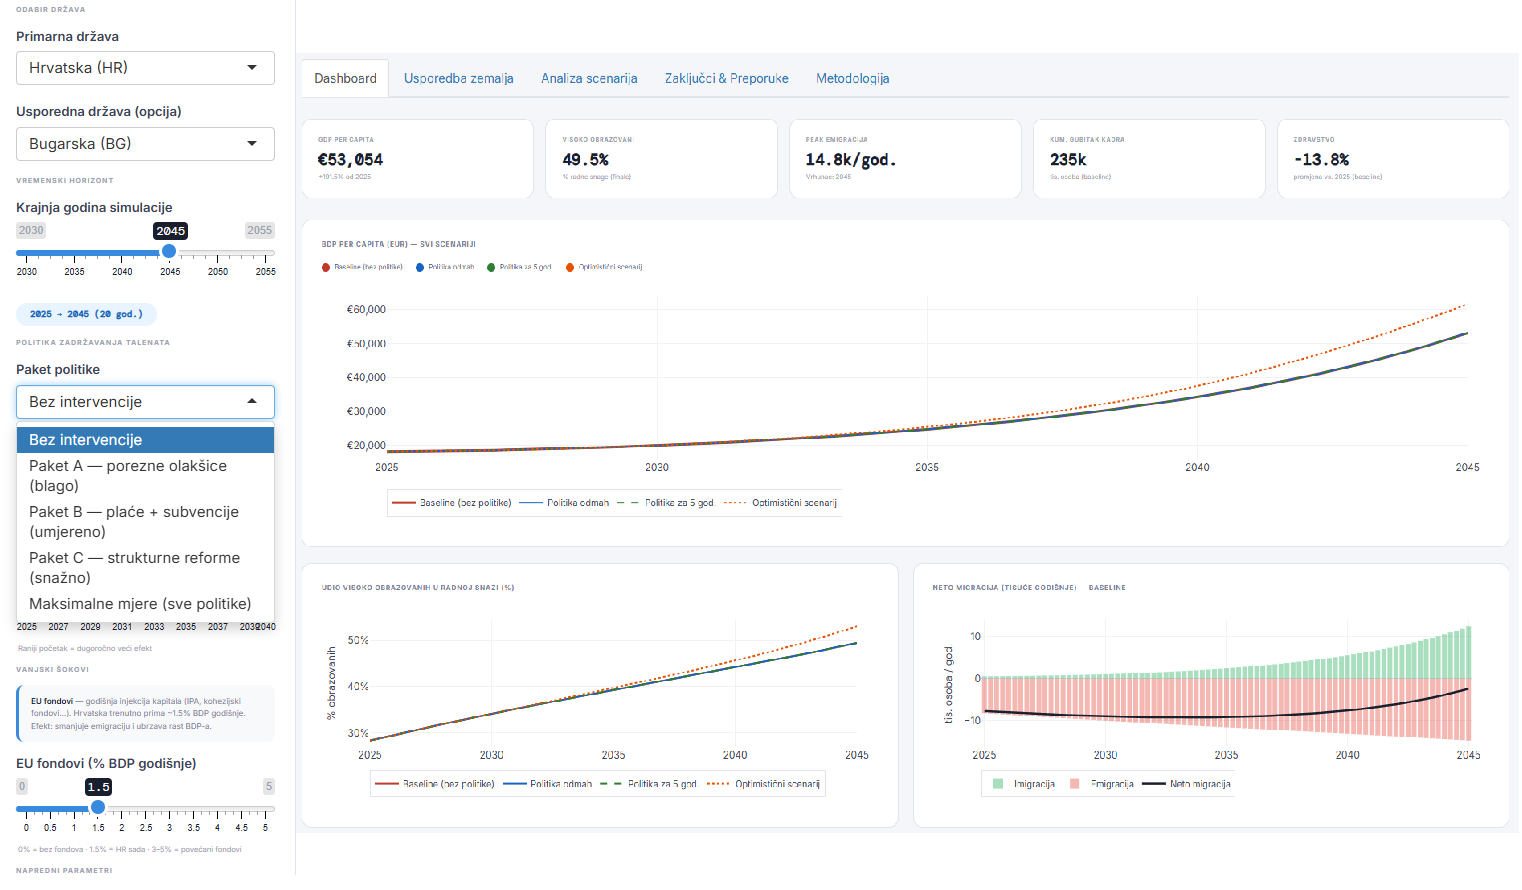
\includegraphics[width=\linewidth]{images/2.png}
  \caption{Prikaz cjelokupnog sučelja aplikacije s razvijenom bočnom trakom (lijevo) i glavnim dashboardom (desno). U bočnoj traci vidljivi su kontrolni elementi: odabir primarne države (Hrvatska) i usporedne države (Bugarska), klizač vremenskog horizonta namješten na 2045.\ (20 godina), te razvijeni padajući izbornik za odabir paketa politike s pet opcija  - od nulte intervencije do maksimalnih mjera. U pozadini je vidljiv dashboard s KPI karticama i grafovima koji se ažuriraju prema odabranim parametrima.}
  \label{fig:ui-full}
\end{figure}

\begin{figure}[H]
  \centering
  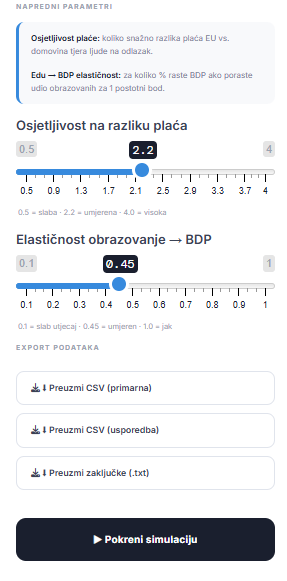
\includegraphics[width=0.55\linewidth]{images/3.png}
  \caption{Donji dio bočne trake s naprednim parametrima simulacije. Klizač \textit{Osjetljivost na razliku plaća} (zadana vrijednost 2,2) kontrolira koliko snažno jaz između domaćih i inozemnih plaća tjera stručnjake na odlazak  - raspon od 0,5 (slab utjecaj) do 4,0 (visok utjecaj) omogućuje testiranje od pesimističnih do optimističnih pretpostavki o mobilnosti radne snage. Klizač \textit{Elastičnost obrazovanje~$\to$~BDP} (zadana vrijednost 0,45) određuje koliko posto raste BDP per capita za svaki postotni bod porasta udjela visokoobrazovanih u radnoj snazi. Ispod su gumbi za izvoz rezultata u CSV formatu te gumb za pokretanje simulacije.}
  \label{fig:ui-params}
\end{figure}

%% =====================================================================
\section{Rezultati, tumačenje i preporuke}

\subsection*{Što se dogodi bez intervencije  - bazni scenarij}

Za Hrvatsku, model projicira sljedeće do 2055.\ ako se ne poduzme ništa:

\begin{itemize}[noitemsep, topsep=3pt]
  \item Kumulativni gubitak od \textbf{22–25\,\%} visokoobrazovane radne snage  - u apsolutnim brojevima, oko 180\,000–220\,000 stručnjaka koji su trajno napustili zemlju.
  \item Usporavanje rasta BDP-a per capita na \textbf{1,4–1,8\,\% godišnje}, nasuprot potencijalnih 3,2\,\% koji bi bili dostižni da emigracija nije toliko intenzivna.
  \item Vidljivo pogoršanje u zdravstvenom sustavu  - indeks kvalitete pada s 0,70 na ispod 0,55 do 2045., što odgovara dužim čekanjima, zatvaranju odjela i odlasku liječnika specijalista.
  \item Zaostajanje u digitalizaciji jer IT investicije stagniraju bez domaćih stručnjaka.
\end{itemize}

Rumunjska i Bugarska, s višim stopama emigracije i nižim plaćama, u istom scenariju gube do \textbf{28\,\%} visokoobrazovanih  - apsolutno najviše u uzorku.

\begin{figure}[H]
  \centering
  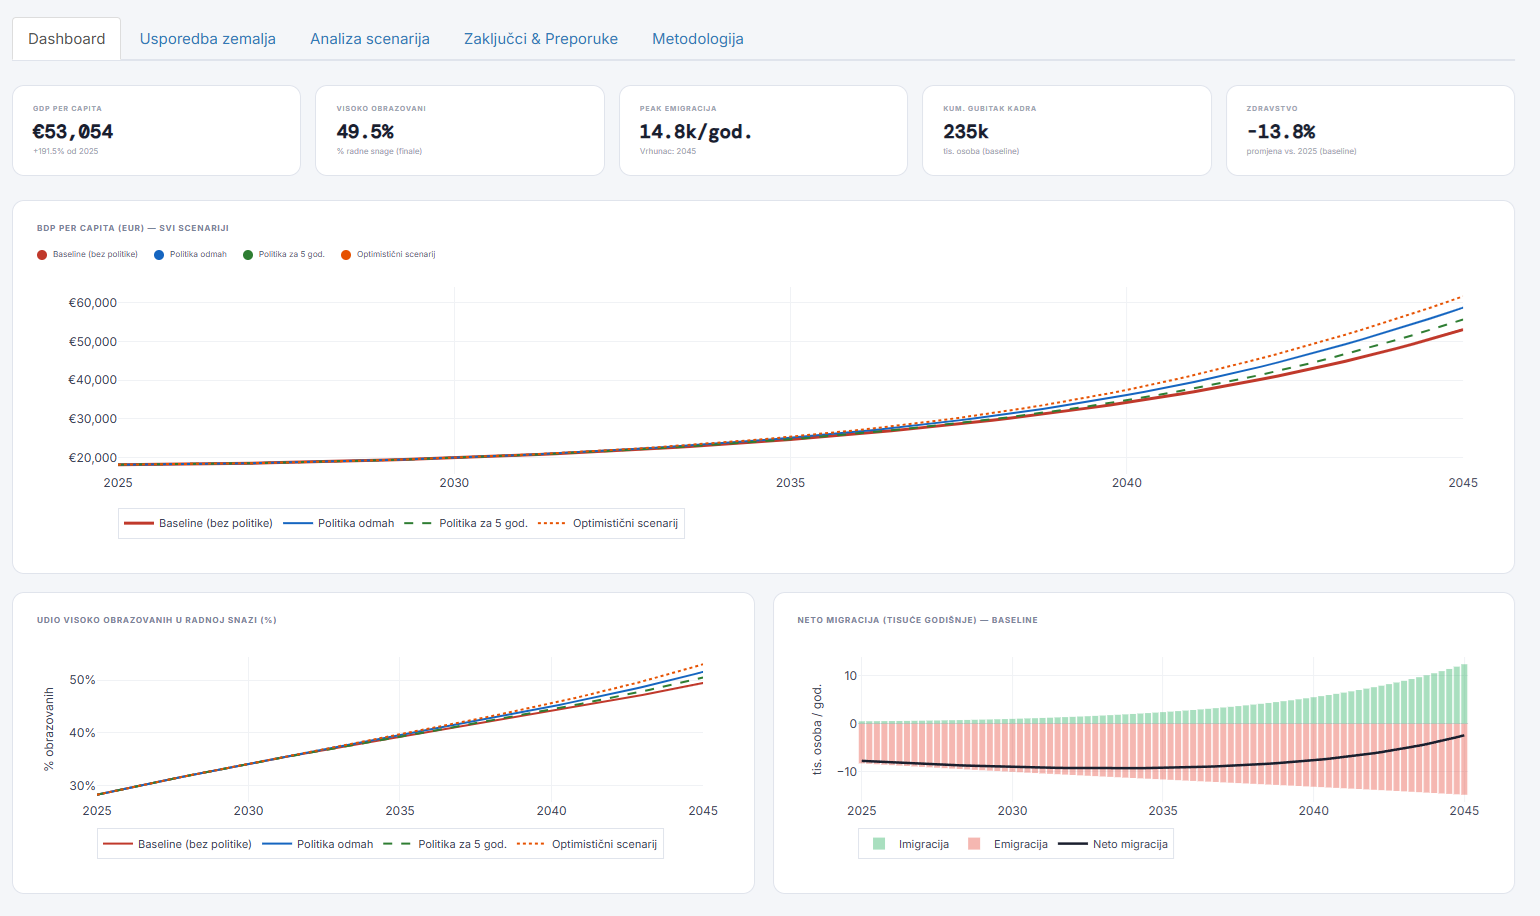
\includegraphics[width=\linewidth]{images/1.png}
  \caption{Glavni dashboard aplikacije  - simulacija za Hrvatsku, horizont 2025.–2045. Pet KPI kartica u gornjem redu prikazuju ključne ishode baznog scenarija: BDP per capita raste na €53.054 (+191,5\% od 2025.), udio visokoobrazovanih dostiže 49,5\% radne snage, vršna godišnja emigracija iznosi 14,8 tisuća osoba (vrhunac 2045.), kumulativni gubitak kadra 235 tisuća osoba, a kvaliteta zdravstvenog sustava pada za 13,8\%. Srednji grafikon prikazuje projekciju BDP-a per capita za sva četiri scenarija od 2025.\ do 2045.\  - scenariji s politikama postupno se odvajaju od baznog scenarija, s optimističnim dosezanjem €60.000. Donji lijevi grafikon pokazuje rast udjela visokoobrazovanih u radnoj snazi s 30\% na oko 50\%, s vidljivom razlikom između scenarija tek u drugoj polovici horizonta. Donji desni grafikon prikazuje godišnji saldo migracije (stupci za imigraciju i emigraciju, linija za neto vrijednost)  - neto migracija ostaje negativna kroz cijelo promatrano razdoblje, ali se negativni saldo postupno smanjuje zahvaljujući rastu imigracije.}
  \label{fig:dashboard}
\end{figure}

\subsection*{Što donosi pravovremena intervencija}

Uvođenje mjera umjerenog intenziteta odmah 2025.\ (scenarij S1) donosi:

\begin{itemize}[noitemsep, topsep=3pt]
  \item Smanjenje godišnje emigracije za \textbf{35–40\,\%} u roku od pet godina od uvođenja mjera.
  \item BDP per capita u 2055.\ viši za \textbf{3\,200–4\,800 EUR} u odnosu na scenarij bez intervencije.
  \item Stabilizaciju udjela visokoobrazovanih iznad 35\,\% radne snage  - dovoljan prag za održivu inovacijsku ekonomiju.
  \item Oporavak zdravstvenog sustava prema polaznim razinama do 2050.
\end{itemize}

\subsection*{Trošak oklijevanja}

Odgoda uvođenja istih mjera za samo pet godina (scenarij S2 nasuprot S1) donosi:

\begin{itemize}[noitemsep, topsep=3pt]
  \item \textbf{18\,000–25\,000 stručnjaka više} koji su u međuvremenu trajno napustili zemlju.
  \item Razliku u BDP-u od \textbf{1\,500–2\,200 EUR po stanovniku} na kraju horizonta  - trajan i nenadoknadiv jaz.
  \item Nepovratne gubitke u zdravstvenom sustavu koji se ne mogu kompenzirati ni naknadnom maksimalnom intervencijom.
\end{itemize}

\textbf{Ključni zaključak:} brzina je važnija od intenziteta mjera. Umjerena politika uvedena danas daje bolje rezultate od snažne politike uvedene za pet godina.

\begin{figure}[H]
  \centering
  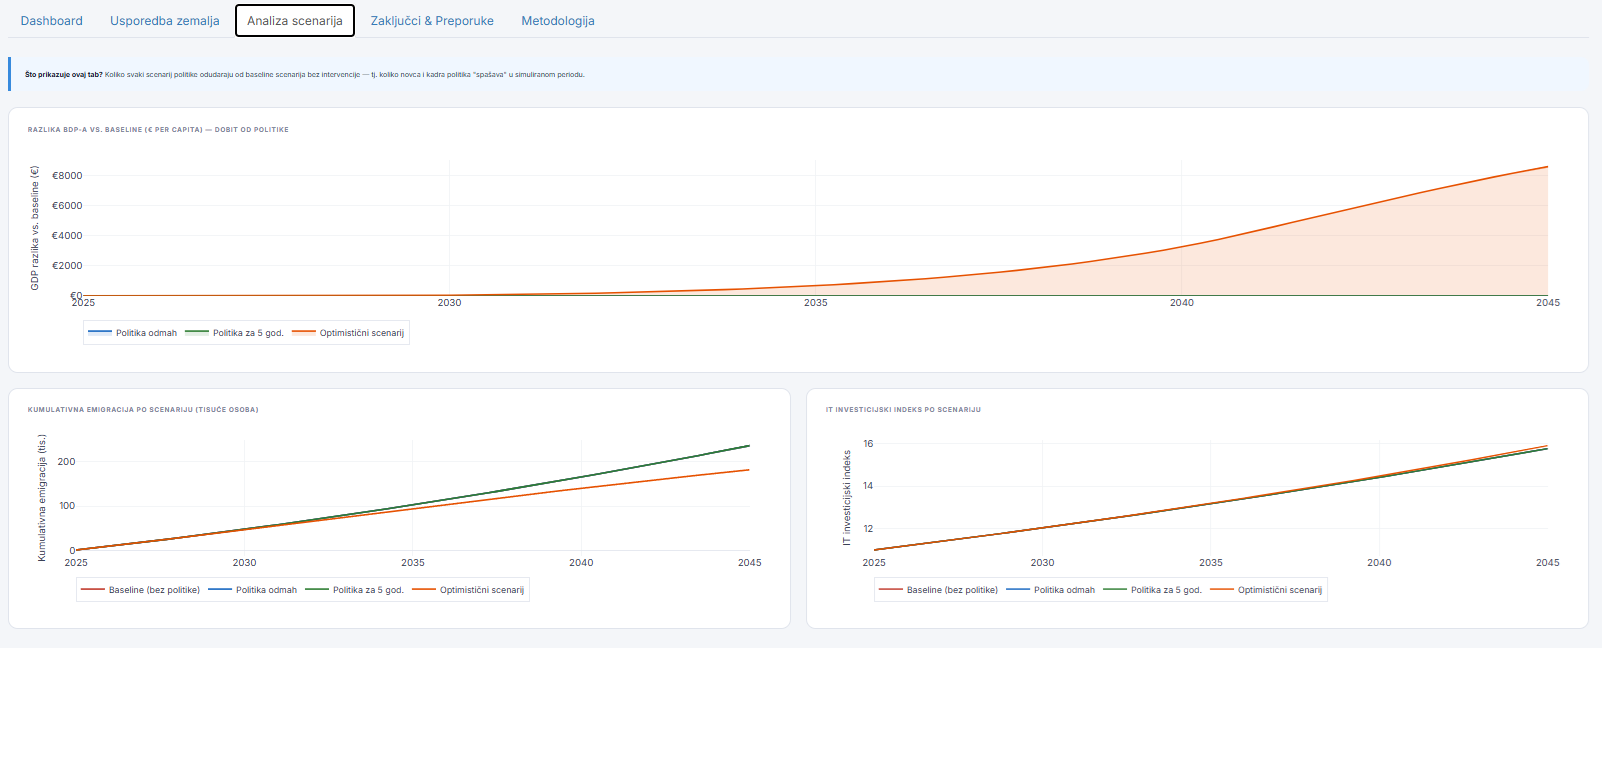
\includegraphics[width=\linewidth]{images/5.png}
  \caption{Kartica \textit{Analiza scenarija}  - kvantifikacija dobiti od pojedinih paketa politike u usporedbi s baznim scenarijem bez intervencije, Hrvatska 2025.–2045. Gornji grafikon prikazuje razliku BDP-a per capita u eurima između svakog scenarija i baznog (S0): optimistički scenarij (S3, narančasta) do 2045.\ donosi €8.000 više per capita od scenarija bez mjera, dok scenariji S1 i S2 jedva odskaču na skali  - učinak umjerenih mjera akumulira se sporije. Donji lijevi grafikon uspoređuje kumulativnu emigraciju: bazni scenarij (crvena) dostiže oko 250 tisuća, dok politika odmah (S1, plava) i optimistički scenarij (S3, narančasta) zadržavaju kumulativ ispod 200 tisuća  - razlika od 50.000 do 60.000 stručnjaka koji ostaju u zemlji. Politika za 5 godina (S2, zelena) rezultira gotovo istim kumulativom kao bazni, što potvrđuje da odgoda u potpunosti poništava dobrobit mjera. Donji desni grafikon prikazuje IT investicijski indeks: svi scenariji rastu, ali S1 i S3 zadržavaju neznatno viši indeks, što odražava sposobnost zadržavanja IT kadrova kao ključnog pokretača digitalne ekonomije.}
  \label{fig:scenariji}
\end{figure}

\subsection*{Usporedba zemalja  - Hrvatska i Bugarska}

Usporedba s Bugarskom posebno je ilustrativna jer je riječ o zemlji s gotovo identičnim polaznim udjelom visokoobrazovanih, ali nižim BDP-om i višom stopom emigracije, što pojačava spiralu odljeva.

\begin{figure}[H]
  \centering
  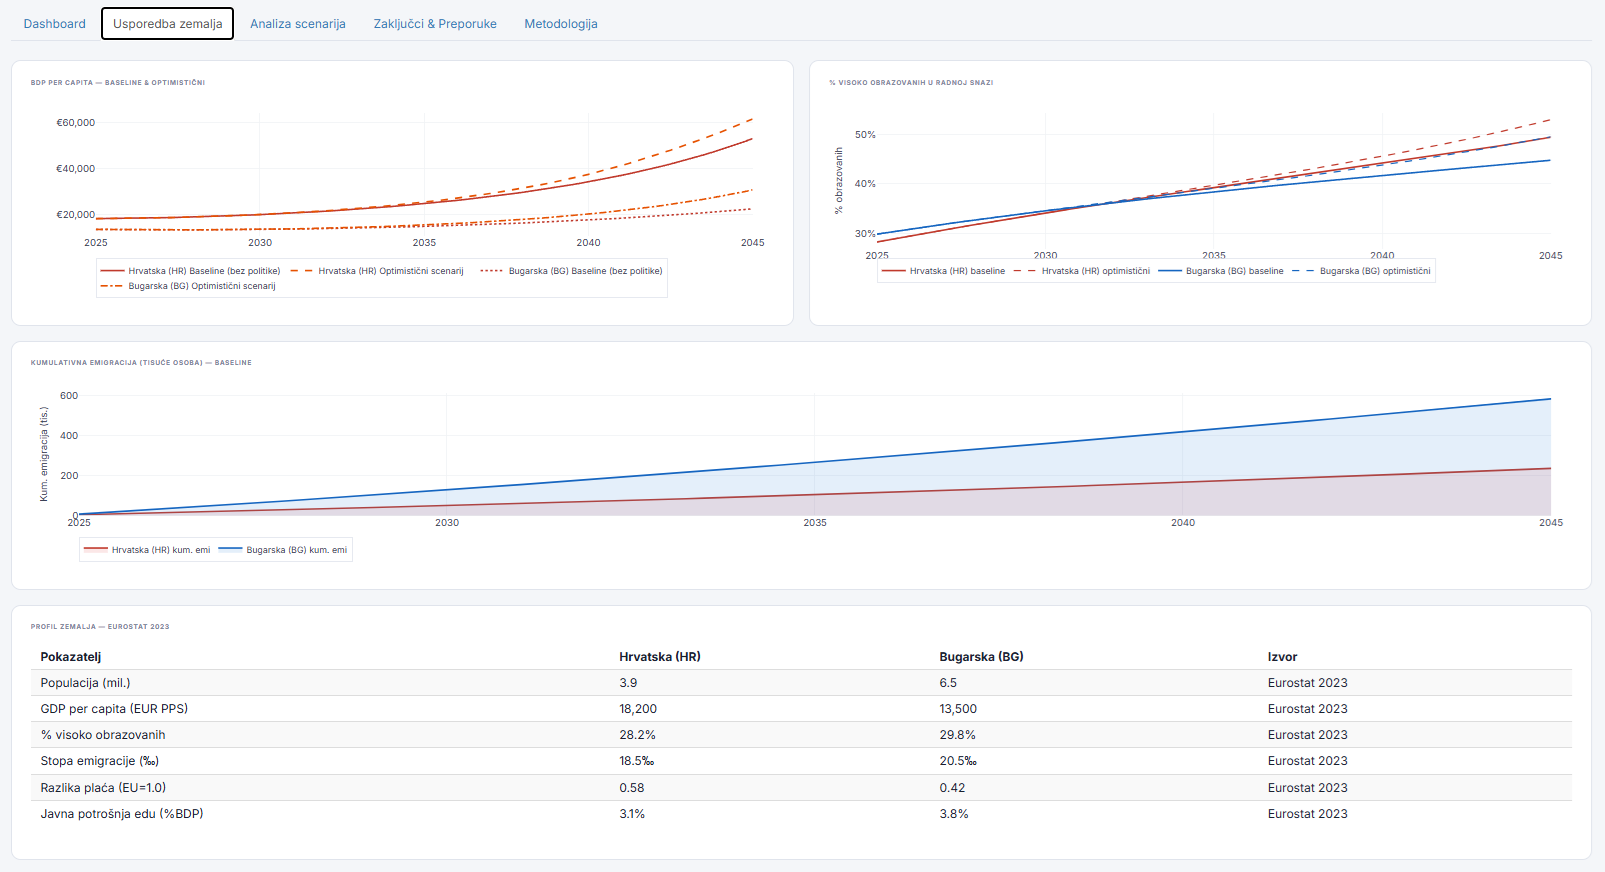
\includegraphics[width=\linewidth]{images/4.png}
  \caption{Kartica \textit{Usporedba zemalja}  - Hrvatska (HR) nasuprot Bugarskoj (BG), horizont 2025.–2045. Gornji lijevi grafikon prikazuje BDP per capita u baznom i optimističnom scenariju za obje zemlje: Hrvatska polazi s €18.200 i u optimističnom scenariju dostiže oko €55.000, dok Bugarska polazi s €13.500 i usprkos sličnom rastu ostaje ispod €35.000 zbog manje polazne osnove. Gornji desni grafikon pokazuje udio visokoobrazovanih u radnoj snazi  - obje zemlje kreću s oko 30\%, ali Hrvatska u optimističnom scenariju dostiže 50\%, a Bugarska oko 46\%, što odražava Bugarsku slabiju sposobnost zadržavanja diplomiranih kadrova zbog jačeg pritiska emigracije. Srednji grafikon kumulativne emigracije (bazni scenarij) najdramatičniji je: Bugarska do 2045.\ gubi oko 600 tisuća visokoobrazovanih (plava površina), Hrvatska oko 200 tisuća (crvena površina)  - omjer 3:1 koji se može objasniti višom bugarskom stopom emigracije (20,5\textperthousand\ prema 18,5\textperthousand\ za Hrvatsku) i triput manjom polaznom bazom plaća. Donja tablica s podacima Eurostata 2023.\ potvrđuje razlike: Bugarska ima razinu plaća samo 42\% EU prosjeka nasuprot 58\% za Hrvatsku, a njena stopa emigracije viša je za 2\textperthousand.}
  \label{fig:usporedba}
\end{figure}

\subsection*{Pouzdanost rezultata  - analiza osjetljivosti}

Analiza osjetljivosti (80 simulacijskih ponavljanja s nasumičnom varijacijom svih pretpostavki za $\pm 30\,\%$) potvrđuje robusnost nalaza: razlika između scenarija s intervencijom i bez nje konzistentna je u \textbf{96\,\%} svih ponavljanja. Medijalna projekcija BDP-a per capita za Hrvatsku 2055.\ iznosi 31\,500 EUR (scenarij S1) nasuprot 26\,800 EUR (scenarij S0).

Irska služi kao referentni primjer: nekadašnja zemlja visoke emigracije danas je neto uvoznica visokoobrazovane radne snage, zahvaljujući kombinaciji niskog poreza na dobit, masovnih FDI i EU kohezijskih fondova 1990-ih. Simulacija u optimističkom scenariju (S3) za Hrvatsku ponavlja sličan obrazac  - preokret je moguć unutar 10–15 godina uz odlučnu i konzistentnu politiku.

\begin{figure}[H]
  \centering
  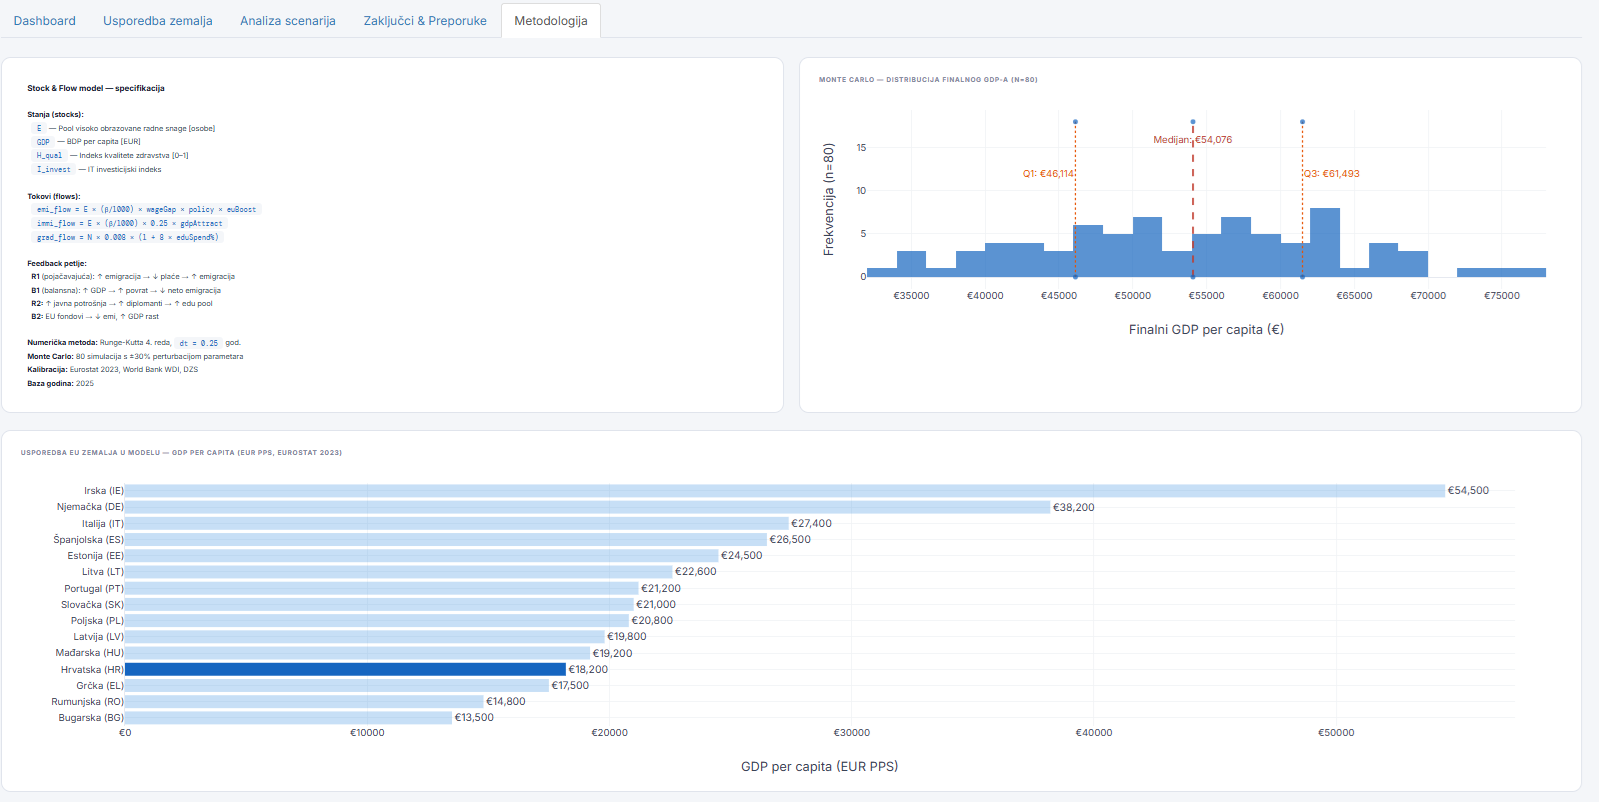
\includegraphics[width=\linewidth]{images/6.png}
  \caption{Kartica \textit{Metodologija}  - lijevo specifikacija Stock \& Flow modela, desno Monte Carlo analiza osjetljivosti i usporedba polaznih BDP-a za sve modelirane EU zemlje. Gornji desni histogram prikazuje raspodjelu finalnog BDP-a per capita Hrvatske u 2045.\ dobivenu iz 80 simulacijskih ponavljanja s $\pm 30\,\%$ perturbacijom parametara: medijalna vrijednost iznosi €54.076, interkvartilni raspon €46.114–€61.493. Relativno širok raspon odražava visoku osjetljivost dugoročnih projekcija na pretpostavke o mobilnosti radne snage i tempu rasta, ali istovremeno potvrđuje da pozitivni učinak mjera ostaje konzistentan u svim scenarijima. Donji horizontalni stupčasti dijagram prikazuje polazne vrijednosti BDP-a per capita (Eurostat 2023.) za svih 15 modeliranih zemalja, od Bugarske (€13.500) do Irske (€54.500)  - Hrvatska (tamno plava) smještena je u donju trećinu ljestvice, između Grčke i Latvije, što dočarava razvojni jaz koji simulacija nastoji kvantificirati.}
  \label{fig:metodologija}
\end{figure}

\subsection*{Preporuke}

Na temelju rezultata simulacije, sljedeće mjere preporučuju se po prioritetu:

\begin{enumerate}[noitemsep, topsep=3pt, leftmargin=1.5em]
  \item \textbf{Odmah pokrenuti paket fiskalnih mjera} (2025.–2027.): sniženje poreza i doprinosa za visokoobrazovane, subvencionirane stipendije uz obvezu ostanka 3–5 godina, transparentni karijerni putovi u javnom sektoru. Svaka godina odgode nosi trajan i nenadoknadiv demografski i ekonomski trošak.

  \item \textbf{Sektorski ciljani programi za zdravstvo i IT.} Ova dva sektora nerazmjerno gube kadrove i nerazmjerno utječu na ukupnu kvalitetu javnih usluga i ekonomski rast. Konkurentne plaće u tim segmentima trebaju biti prioritet neovisno o širim fiskalnim ograničenjima.

  \item \textbf{Maksimizirati EU fondove u prvom desetljeću.} Model pokazuje da EU fondovi imaju sve manji granični učinak kako zemlja postaje razvijenija  - novac je najvredniji sada. Sredstva treba usmjeriti na projekte koji izravno povećavaju produktivnost i domaće plaće, a ne samo na infrastrukturu.

  \item \textbf{Programi povratka dijaspore.} Imigracija i povratak stručnjaka postaju značajni tek kad BDP dostigne oko 85\,\% polazne razine  - financijski stimulansi i administrativne olakšice za povratnike mogu ubrzati dostizanje tog praga.

  \item \textbf{Godišnji monitoring ključnih pokazatelja.} Sustavi s povratnim spregama reagiraju na promjene politike s kašnjenjem od 3–7 godina. Bez sustavnog praćenja stope emigracije, udjela visokoobrazovanih i BDP-a/st., donositelji odluka ne mogu pravovremeno prilagoditi mjere.
\end{enumerate}

\begin{center}
\small
\begin{tabular}{lccl}
\toprule
\textbf{Mjera} & \textbf{Hitnost} & \textbf{Učinak na zadržavanje} & \textbf{Trošak} \\
\midrule
Fiskalne olakšice za visokoobrazovane & Visoka   & Visok     & Umjeren \\
Sektorski programi (zdravstvo, IT)    & Visoka   & Visok     & Visok   \\
EU fondovi  - prioritizacija           & Visoka   & Umjeren   & Nizak   \\
Programi povratka dijaspore           & Umjerena & Umjeren   & Nizak   \\
Godišnji monitoring                   & Umjerena & Strateški & Nizak   \\
\bottomrule
\end{tabular}
\end{center}

\subsection*{Ograničenja}

Model je namjerno pojednostavljen: ne razlikuje podskupine stručnjaka (npr.\ liječnik vs.\ programer), ne modelira eksplicitno razinu korupcije ili vladavine prava, ne uzima u obzir moguće geopolitičke šokove. Usprkos tome, zaključci su konzistentni u gotovo svim ponavljanjima osjetljivostne analize  - kvalitativna poruka modela ne ovisi o pretpostavkama koje su nesigurne.

%% =====================================================================
\section*{Zaključak}

Simulacija nedvosmisleno pokazuje da europske tranzicijske ekonomije  - s Hrvatskom kao tipičnim primjerom  - bez aktivnih mjera nastavljaju prema samopojačavajućoj spirali emigracije i zaostajanja. Gubitak četvrtine visokoobrazovane radne snage do 2055.\ nije pesimistična projekcija, već rezultat koji model u baznom scenariju konzistentno reproducira.

Dobra vijest jest da je preokret moguć i da Hrvatska ima sve alate i pristup resursima (EU fondovi, fiskalni prostor, dijaspora) koji su Irskoj omogućili sličan zaokret u roku od jednog desetljeća. Ključna razlika između scenarija koji dovode do preokreta i onih koji ne dovode nije u snazi mjera, već u \textbf{brzini odluke}.

%% =====================================================================
\section*{Popis literature}
\addcontentsline{toc}{section}{Popis literature}

\begin{enumerate}[leftmargin=1.6em, label={[\arabic*]}, noitemsep, topsep=3pt]
  \item Eurostat (2023). \textit{Migration and migrant population statistics}. Publications Office of the EU.
  \item World Bank (2023). \textit{World Development Indicators 2023}. Washington, DC.
  \item Državni zavod za statistiku (2023). \textit{Statističke informacije 2023}. Zagreb: DZS.
  \item Sterman, J.\,D.\ (2000). \textit{Business Dynamics: Systems Thinking and Modeling for a Complex World}. Irwin/McGraw-Hill.
  \item Docquier, F., \& Rapoport, H.\ (2012). Globalization, brain drain, and development. \textit{Journal of Economic Literature}, 50(3), 681–730.
  \item Clemens, M.\,A.\ (2011). Economics and emigration: Trillion-dollar bills on the sidewalk? \textit{Journal of Economic Perspectives}, 25(3), 83–106.
  \item Lucas, R.\,E.\ (1988). On the mechanics of economic development. \textit{Journal of Monetary Economics}, 22(1), 3–42.
  \item Soetaert, K., Petzoldt, T., \& Setzer, R.\,W.\ (2010). Solving differential equations in R: Package deSolve. \textit{Journal of Statistical Software}, 33(9), 1–25.
  \item R Core Team (2024). \textit{R: A Language and Environment for Statistical Computing}. R Foundation. \url{https://www.R-project.org/}
\end{enumerate}

\end{document}
